\PassOptionsToPackage{unicode=true}{hyperref} % options for packages loaded elsewhere
\PassOptionsToPackage{hyphens}{url}
\PassOptionsToPackage{dvipsnames,svgnames*,x11names*}{xcolor}
%
\documentclass[]{article}
\usepackage{lmodern}
\usepackage{amssymb,amsmath}
\usepackage{ifxetex,ifluatex}
\usepackage{fixltx2e} % provides \textsubscript
\ifnum 0\ifxetex 1\fi\ifluatex 1\fi=0 % if pdftex
  \usepackage[T1]{fontenc}
  \usepackage[utf8]{inputenc}
  \usepackage{textcomp} % provides euro and other symbols
\else % if luatex or xelatex
  \usepackage{unicode-math}
  \defaultfontfeatures{Ligatures=TeX,Scale=MatchLowercase}
\fi
% use upquote if available, for straight quotes in verbatim environments
\IfFileExists{upquote.sty}{\usepackage{upquote}}{}
% use microtype if available
\IfFileExists{microtype.sty}{%
\usepackage[]{microtype}
\UseMicrotypeSet[protrusion]{basicmath} % disable protrusion for tt fonts
}{}
\IfFileExists{parskip.sty}{%
\usepackage{parskip}
}{% else
\setlength{\parindent}{0pt}
\setlength{\parskip}{6pt plus 2pt minus 1pt}
}
\usepackage{xcolor}
\usepackage{hyperref}
\hypersetup{
            pdftitle={Matemáticas III GIN ejercicios para entrenar 1},
            colorlinks=true,
            linkcolor=Maroon,
            filecolor=Maroon,
            citecolor=Blue,
            urlcolor=blue,
            breaklinks=true}
\urlstyle{same}  % don't use monospace font for urls
\usepackage[margin=1in]{geometry}
\usepackage{color}
\usepackage{fancyvrb}
\newcommand{\VerbBar}{|}
\newcommand{\VERB}{\Verb[commandchars=\\\{\}]}
\DefineVerbatimEnvironment{Highlighting}{Verbatim}{commandchars=\\\{\}}
% Add ',fontsize=\small' for more characters per line
\usepackage{framed}
\definecolor{shadecolor}{RGB}{248,248,248}
\newenvironment{Shaded}{\begin{snugshade}}{\end{snugshade}}
\newcommand{\AlertTok}[1]{\textcolor[rgb]{0.94,0.16,0.16}{#1}}
\newcommand{\AnnotationTok}[1]{\textcolor[rgb]{0.56,0.35,0.01}{\textbf{\textit{#1}}}}
\newcommand{\AttributeTok}[1]{\textcolor[rgb]{0.77,0.63,0.00}{#1}}
\newcommand{\BaseNTok}[1]{\textcolor[rgb]{0.00,0.00,0.81}{#1}}
\newcommand{\BuiltInTok}[1]{#1}
\newcommand{\CharTok}[1]{\textcolor[rgb]{0.31,0.60,0.02}{#1}}
\newcommand{\CommentTok}[1]{\textcolor[rgb]{0.56,0.35,0.01}{\textit{#1}}}
\newcommand{\CommentVarTok}[1]{\textcolor[rgb]{0.56,0.35,0.01}{\textbf{\textit{#1}}}}
\newcommand{\ConstantTok}[1]{\textcolor[rgb]{0.00,0.00,0.00}{#1}}
\newcommand{\ControlFlowTok}[1]{\textcolor[rgb]{0.13,0.29,0.53}{\textbf{#1}}}
\newcommand{\DataTypeTok}[1]{\textcolor[rgb]{0.13,0.29,0.53}{#1}}
\newcommand{\DecValTok}[1]{\textcolor[rgb]{0.00,0.00,0.81}{#1}}
\newcommand{\DocumentationTok}[1]{\textcolor[rgb]{0.56,0.35,0.01}{\textbf{\textit{#1}}}}
\newcommand{\ErrorTok}[1]{\textcolor[rgb]{0.64,0.00,0.00}{\textbf{#1}}}
\newcommand{\ExtensionTok}[1]{#1}
\newcommand{\FloatTok}[1]{\textcolor[rgb]{0.00,0.00,0.81}{#1}}
\newcommand{\FunctionTok}[1]{\textcolor[rgb]{0.00,0.00,0.00}{#1}}
\newcommand{\ImportTok}[1]{#1}
\newcommand{\InformationTok}[1]{\textcolor[rgb]{0.56,0.35,0.01}{\textbf{\textit{#1}}}}
\newcommand{\KeywordTok}[1]{\textcolor[rgb]{0.13,0.29,0.53}{\textbf{#1}}}
\newcommand{\NormalTok}[1]{#1}
\newcommand{\OperatorTok}[1]{\textcolor[rgb]{0.81,0.36,0.00}{\textbf{#1}}}
\newcommand{\OtherTok}[1]{\textcolor[rgb]{0.56,0.35,0.01}{#1}}
\newcommand{\PreprocessorTok}[1]{\textcolor[rgb]{0.56,0.35,0.01}{\textit{#1}}}
\newcommand{\RegionMarkerTok}[1]{#1}
\newcommand{\SpecialCharTok}[1]{\textcolor[rgb]{0.00,0.00,0.00}{#1}}
\newcommand{\SpecialStringTok}[1]{\textcolor[rgb]{0.31,0.60,0.02}{#1}}
\newcommand{\StringTok}[1]{\textcolor[rgb]{0.31,0.60,0.02}{#1}}
\newcommand{\VariableTok}[1]{\textcolor[rgb]{0.00,0.00,0.00}{#1}}
\newcommand{\VerbatimStringTok}[1]{\textcolor[rgb]{0.31,0.60,0.02}{#1}}
\newcommand{\WarningTok}[1]{\textcolor[rgb]{0.56,0.35,0.01}{\textbf{\textit{#1}}}}
\usepackage{longtable,booktabs}
% Fix footnotes in tables (requires footnote package)
\IfFileExists{footnote.sty}{\usepackage{footnote}\makesavenoteenv{longtable}}{}
\usepackage{graphicx,grffile}
\makeatletter
\def\maxwidth{\ifdim\Gin@nat@width>\linewidth\linewidth\else\Gin@nat@width\fi}
\def\maxheight{\ifdim\Gin@nat@height>\textheight\textheight\else\Gin@nat@height\fi}
\makeatother
% Scale images if necessary, so that they will not overflow the page
% margins by default, and it is still possible to overwrite the defaults
% using explicit options in \includegraphics[width, height, ...]{}
\setkeys{Gin}{width=\maxwidth,height=\maxheight,keepaspectratio}
\setlength{\emergencystretch}{3em}  % prevent overfull lines
\providecommand{\tightlist}{%
  \setlength{\itemsep}{0pt}\setlength{\parskip}{0pt}}
\setcounter{secnumdepth}{0}
% Redefines (sub)paragraphs to behave more like sections
\ifx\paragraph\undefined\else
\let\oldparagraph\paragraph
\renewcommand{\paragraph}[1]{\oldparagraph{#1}\mbox{}}
\fi
\ifx\subparagraph\undefined\else
\let\oldsubparagraph\subparagraph
\renewcommand{\subparagraph}[1]{\oldsubparagraph{#1}\mbox{}}
\fi

% set default figure placement to htbp
\makeatletter
\def\fps@figure{htbp}
\makeatother


\title{Matemáticas III GIN ejercicios para entrenar 1}
\author{}
\date{\vspace{-2.5em}}

\begin{document}
\maketitle

{
\hypersetup{linkcolor=}
\setcounter{tocdepth}{2}
\tableofcontents
}
\begin{verbatim}
## Warning: package 'knitr' was built under R version 3.6.2
\end{verbatim}

\hypertarget{matemuxe1ticas-iii.-algunos-ejercicios-para-entrenar-tipo-examen-de-los-temas-de-probabilidad-variables-aleatorias-y-distribuciones-notables}{%
\section{Matemáticas III. Algunos EJERCICIOS para ENTRENAR tipo examen;
de los temas de: Probabilidad, Variables Aleatorias y Distribuciones
Notables}\label{matemuxe1ticas-iii.-algunos-ejercicios-para-entrenar-tipo-examen-de-los-temas-de-probabilidad-variables-aleatorias-y-distribuciones-notables}}

\hypertarget{ejercicio-1}{%
\subsection{Ejercicio 1}\label{ejercicio-1}}

Sean \(A\) y \(B\) dos sucesos tales que
\(P(A\cap B^c)=P(B\cap A^c)=P(A\cap B)=0.2\) ¿Qué vale \(P(A\cup B)\)?

\hypertarget{soluciuxf3n}{%
\subsubsection{Solución:}\label{soluciuxf3n}}

Tenemos que \(P(A\cap B^c)=P(A-B)=P(A)-P(A\cap B)=0.2\) y también
\(P(B\cap A^c)=P(B-A)=P(B)-P(A\cap B)=0.2\). De donde, utilizando que
\(P(A\cap B)=0.2\) tenemos que \(P(A)=P(B)=0.4\). Y ahora calculamos lo
que se pide \[P(A\cup B)=P(A)+P(B)-P(A\cap B)=0.4+0.4-0.2=0.6.\]

\hypertarget{ejercicio-2}{%
\subsection{Ejercicio 2}\label{ejercicio-2}}

En una muestra aleatoria simple de tamaño \(100\) de la población de
internautas se obtuvo que el 80\% tenían cuenta en al menos dos redes
sociales. Calcular el error estándar de la proporción \(p\) de
internautas que tienen cuenta el al menos dos redes sociales.

\hypertarget{soluciuxf3n-1}{%
\subsubsection{Solución:}\label{soluciuxf3n-1}}

Tenemos una muestra aleatoria simple de tamaño \(n=100\) en la que la
proporción muestral es \(\hat{p}=0.8\). Bajo estas condiciones el error
estándar del estadístico \(\hat{p}\) es

\[\sqrt{\frac{\hat{p}\cdot (1- \hat{p})}{n}}=\sqrt{\frac{0.8\cdot (0.2)}{ n}}=0.04.\]

\hypertarget{ejercicio-3}{%
\subsection{Ejercicio 3}\label{ejercicio-3}}

¿Cuál es la probabilidad de que la suma de los puntos de dos dados de
parchís perfectos sea \(7\) en los siguientes tres casos?

a). Tiro un dado dos veces y sumo los resultados.

b). Tiro a la vez dos dados blancos y sumo los resultados.

c). Tiro a la vez un dado rojo y uno azul y sumo los resultados.

\hypertarget{soluciuxf3n-2}{%
\subsubsection{Solución:}\label{soluciuxf3n-2}}

En las tres situaciones a), b) y c) los casos posibles son los
siguientes pares dónde el primer elemento es el Dado1 (sea del color que
sea) y el segundo es el Dado 2 (de cualquier color)
\(\{(1,6),(2,5),(3,4),(4,3),(5,2),(6,1)\}\).

Así que
\(P( \mbox{La suma es } 7)=\frac{\mbox{Casos Favorables}}{\mbox{Casos Posibles}}=\frac{6}{36}=\frac{1}{6}\)

\hypertarget{ejercicio-4}{%
\subsection{Ejercicio 4}\label{ejercicio-4}}

Sea \(X\) una variable aleatoria que cuenta el número de \textbf{CARAS}
de una moneda trucada una distribución \(B(n=100,p=\frac{1}{4})\).
Sabemos que \(P(X\leq 40)=0.8962\) ¿Cuál es la probabilidad de obtener
\(59\) \textbf{CRUCES} o menos? (Indicación construid la variable
\(Y=100-X\) que cuenta el número de \textbf{CRUCES}.)

\hypertarget{soluciuxf3n-3}{%
\subsubsection{Solución:}\label{soluciuxf3n-3}}

Sea \(Y\) la variable que cuenta el número de cruces en el mismo
experimento. Obviamente tenemos que \(Y=100-X\). Así que

\[P(Y=59)= P(100-X\leq 59) = P(X\geq 41)= 1-P(X < 41)=1-P(X\leq 40)=1-0.8962=0.1038.\]

\hypertarget{ejercicio-5}{%
\subsection{Ejercicio 5}\label{ejercicio-5}}

Si \(X\) es una variable aleatoria con distribución \(Exp(\lambda)\) y
sabemos que \(P(X>4)=0.5\) ¿Qué vale \(P(X\geq 8/X>4)\)?

\hypertarget{soluciuxf3n-4}{%
\subsubsection{Solución:}\label{soluciuxf3n-4}}

Sabemos que la distribución exponencial carece de memoria lo que quiere
decir que \(P(X> x+y/X>x)=P(X> y)\). En nuestro caso

\[P(X>8/X>4)=P(X> 4+4/X>4)=P(X>4)=0.5.\]

\hypertarget{ejercicio-6}{%
\subsection{Ejercicio 6}\label{ejercicio-6}}

Cuatro personas con cuatro gorras diferentes las lanzan al aire para
celebrar la victoria de su equipo. Cuando caen las recogen al azar.
Estudiar la distribución de la variable que nos da el número de gorras
que se quedan con su dueño (\textbf{1 punto}).

\hypertarget{soluciuxf3n-5}{%
\subsubsection{Solución:}\label{soluciuxf3n-5}}

\begin{Shaded}
\begin{Highlighting}[]
\KeywordTok{library}\NormalTok{(combinat)}
\end{Highlighting}
\end{Shaded}

\begin{verbatim}
## 
## Attaching package: 'combinat'
\end{verbatim}

\begin{verbatim}
## The following object is masked from 'package:utils':
## 
##     combn
\end{verbatim}

\begin{Shaded}
\begin{Highlighting}[]
\NormalTok{Casos=}\KeywordTok{as.data.frame}\NormalTok{(}\KeywordTok{matrix}\NormalTok{(}\KeywordTok{unlist}\NormalTok{(}\KeywordTok{permn}\NormalTok{(}\DecValTok{1}\OperatorTok{:}\DecValTok{4}\NormalTok{)),}\DataTypeTok{byrow=}\OtherTok{TRUE}\NormalTok{,}\DataTypeTok{ncol=}\DecValTok{4}\NormalTok{))}
\KeywordTok{names}\NormalTok{(Casos)=}\KeywordTok{paste}\NormalTok{(}\StringTok{"Persona"}\NormalTok{,}\DecValTok{1}\OperatorTok{:}\DecValTok{4}\NormalTok{,}\DataTypeTok{sep=}\StringTok{""}\NormalTok{)}
\NormalTok{Casos}\OperatorTok{$}\NormalTok{Aciertos=}\KeywordTok{unlist}\NormalTok{(}\KeywordTok{apply}\NormalTok{(Casos[,}\DecValTok{1}\OperatorTok{:}\DecValTok{4}\NormalTok{],}\DataTypeTok{MARGIN=}\DecValTok{1}\NormalTok{,}\DataTypeTok{FUN=}\ControlFlowTok{function}\NormalTok{(x) }\KeywordTok{sum}\NormalTok{(x}\OperatorTok{==}\KeywordTok{c}\NormalTok{(}\DecValTok{1}\OperatorTok{:}\DecValTok{4}\NormalTok{))))}
\NormalTok{Casos}
\end{Highlighting}
\end{Shaded}

\begin{verbatim}
##    Persona1 Persona2 Persona3 Persona4 Aciertos
## 1         1        2        3        4        4
## 2         1        2        4        3        2
## 3         1        4        2        3        1
## 4         4        1        2        3        0
## 5         4        1        3        2        1
## 6         1        4        3        2        2
## 7         1        3        4        2        1
## 8         1        3        2        4        2
## 9         3        1        2        4        1
## 10        3        1        4        2        0
## 11        3        4        1        2        0
## 12        4        3        1        2        0
## 13        4        3        2        1        0
## 14        3        4        2        1        0
## 15        3        2        4        1        1
## 16        3        2        1        4        2
## 17        2        3        1        4        1
## 18        2        3        4        1        0
## 19        2        4        3        1        1
## 20        4        2        3        1        2
## 21        4        2        1        3        1
## 22        2        4        1        3        0
## 23        2        1        4        3        0
## 24        2        1        3        4        2
\end{verbatim}

\begin{Shaded}
\begin{Highlighting}[]
\KeywordTok{table}\NormalTok{(Casos}\OperatorTok{$}\NormalTok{Aciertos)}
\end{Highlighting}
\end{Shaded}

\begin{verbatim}
## 
## 0 1 2 4 
## 9 8 6 1
\end{verbatim}

Sea \(X=\) número de personas con su propio sombrero, el dominio es
\(D_X=\{0,1,2,3,4\}\).

Como son equiprobables y los casos posibles son \(4!=24\) tenemos que

\[P(X=k)=\frac{\mbox{Casos favorables a $k$ aciertos}}{\mbox{Casos posibles}}=\frac{\mbox{Casos favorables a k aciertos}}{24}\]

Contando los casos tenemos que

\begin{longtable}[]{@{}rr@{}}
\toprule
Aciertos & Frecuencia\tabularnewline
\midrule
\endhead
0 & 9\tabularnewline
1 & 8\tabularnewline
2 & 6\tabularnewline
4 & 1\tabularnewline
\bottomrule
\end{longtable}

por lo tanto \[P(X=k)=\left\{
\begin{array}{lr}
\frac{9}{24} & k=0\\
\frac{8}{24} & k=1\\
\frac{6}{24} & k=2\\
\frac{1}{24} & k=4\\
0 & \mbox{en otro caso}
\end{array}
\right.
\]

Calculemos la esperanza y la varianza

\(E(X)= 0\cdot \frac{9}{24} +1\cdot \frac{8}{24} + 2 \cdot \frac{6}{24} + 4 \cdot \frac{1}{24} =\frac{8+12+4}{24}=1\)

\(E(X^2)= 0\cdot \frac{9}{24} +1^2\cdot \frac{8}{24} + 2^2 \cdot \frac{6}{24} + 4^2 \cdot \frac{1}{24} =\frac{8+24+16}{24}=2\)

\(Var(X)=E(X^2)-E(X)^2=2-1^2=1\).

\hypertarget{ejercicio-7}{%
\subsection{Ejercicio 7}\label{ejercicio-7}}

Diseñamos un examen tipo test de \(n=10\) preguntas con \(k>2\) opciones
cada una de la que sólo una es correcta. Cada pregunta vale un punto.
Supongamos que un estudiante contesta todas las preguntas al azar. Se
pide

a). Si cada pregunta vale un punto y cada fallo 0 puntos ¿Cuál es el
valor esperado de la nota del estudiante en función de \(k\)?
(\textbf{0.5 puntos}).

b). En función de \(k\) ¿cuál es la el valor que tenemos que asignar a
cada respuesta incorrecta para que la nota esperada del estudiante que
contesta al azar sea \(0\)? (\textbf{0.5 puntos})

c). Puntuando como decidáis en el apartado anterior ¿Cuál es la varianza
de la nota de un estudiante que contesta al azar?(\textbf{0.5 puntos})

\hypertarget{soluciuxf3n-6}{%
\subsubsection{Solución:}\label{soluciuxf3n-6}}

Sea \(X\) el número de preguntas que acierta el estudiante que contesta
al azar. Tiene como probabilidad de acertar \(p=\frac{1}{4}\). Como
contesta al azar y de forma independiente cada pregunta \(X\) sigue una
distribución \(B(n=10,p=\frac{1}{k})\).

La nota es \(N=1\cdot X\). Así que el valor esperado es
\(E(N)=E(X)=n\cdot p=\frac{10}{k}.\)

Ahora puntuamos restando \(c\) por cada pregunta incorrecta. Entonces la
nota es \(N=X+c (10-X)=(1-c) X+10\cdot c\). Por lo tanto el valor
esperado es

\[E(N)=E((1-c) X+10\cdot  c)=(1-c) E(X)+10\cdot c=(1-c)\frac{10}{k}+10\cdot c.\]

Así que el valor \(c\) que hace la esperanza cero debe cumplir

\[0=E(X)=(1-c)\frac{10}{k}+10\cdot c\]

de donde obtenemos que \(c=-\frac{1}{k-1}\).

Así que la nota penalizando es
\(N=\left(1+\frac{1}{k-1}\right) X-\frac{10}{k-1}.\)

Ahora nos piden la varianza de la nota cuando penalizamos las respuestas
incorrectas

\(Var(N)=Var\left(\left(1+\frac{1}{k-1}\right) X-10\cdot\frac{1}{k-1}\right)=\left(1+\frac{1}{k-1}\right)^2 Var(X)= \left(1+\frac{1}{k-1}\right)^2\cdot 10\cdot \frac{1}{k} \left(1-\frac{1}{k}\right)=\frac{10}{k-1}.\)

\hypertarget{ejercicio-8}{%
\subsection{Ejercicio 8}\label{ejercicio-8}}

Consideremos la función de densidad de una cierta variable continua
\(X\)

\[f(x)=\left\{
\begin{array}{cr}
-k\cdot x & \mbox{ si } -1<x<0\\
k\cdot x & \mbox{ si }  0<x<1\\
0 & \mbox{ en cualquier otro caso}
\end{array}
\right.
\]

Se pide

a). Calcular \(k\). (\textbf{0.5 puntos})

b). Calcular la función de distribución de \(X\). (\textbf{0.5 puntos})

c). Calcular \(Var(X)\). (\textbf{0.5 puntos})

\hypertarget{soluciuxf3n-7}{%
\subsubsection{Solución:}\label{soluciuxf3n-7}}

Para calcular utilizaremos que una densidad es positiva y que
\(\int_{-\infty}^{\infty} f(x) dx=1\).

Por lo tanto tenemos que

\(1=\int_{-\infty}^{\infty} f(x) dx=\int_{-1}^{1} f(x) dx= \int_{-1}^{0} -k \cdot x dx+\int_{0}^{1} k \cdot x dx= \left[-k\frac{x^2}{2}\right]_{x=-1}^0+\left[k\frac{x^2}{2}\right]_{x=0}^1= 0- \frac{-k}{2}+ \frac{k}{2}-0=k\)

Por lo tanto \(k=1\)

Así que la función de densidad es \[f(x)=\left\{
\begin{array}{cr}
|x| & \mbox{ si }  -1<x<1\\
0 & \mbox{ en cualquier otro caso}
\end{array}
\right.
\] Calculemos su función de distribución

\[F(X)=P(X\leq x)=\left\{
\begin{array}{lr}
0 & \mbox{ si }  x\leq -1\\
\int_{-1}^x |t| dt=\int_{-1}^x -t dt=\left[-\frac{t^2}{2}\right]_{t=-1}^x= \frac{-x^2}{2}-\frac{-1}{2}=\frac{1-x^2}{2}   & \mbox{ si }  -1< x <0\\
\int_{-1}^x |t| dt=\int_{-1}^{0} -t dt +\int_{0}^x t dt=\frac{1}{2}+\left[\frac{t^2}{2}\right]_{t=0}^x= \frac{1}{2}+\frac{x^2}{2}-0=\frac{x^2+1}{2}   & \mbox{ si }  0\leq x\leq 1\\
\qquad 1 & \mbox{si } x \geq 1
\end{array}
\right.
.\]

En definitiva la función de distribución es

\[
F(X)=P(X\leq x)=\left\{
\begin{array}{lr}
0 & \mbox{ si }  x\leq -1\\
\frac{x^2-1}{2}   & \mbox{ si }  -1< x <0\\
\frac{x^2+1}{2}   & \mbox{ si }  0 \leq x\leq 1\\
1 & \mbox{si } x \geq 1
\end{array}
\right.
.
\]

El valor esperado es

\[E(X)=\int_{-1}^{0} x\cdot (-x) dx+\int_{0}^{1} x\cdot x dx= \left[-\frac{x^3}{3}\right]_{x=-1}^0+
\left[\frac{x^3}{3}\right]_ {x=0}^1=0.
\]

y la varianza

\[Var(X)=E(X^2)-E(X)^2=\int_{-1}^{0} x^2\cdot (-x) dx+\int_{0}^{1} x^2\cdot x dx-0=
\left[-\frac{x^4}{4}\right]_{x=-1}^0+\left[\frac{x^4}{4}\right]_{x=0}^1=0-\frac{-1}{4}+\frac{1}{4}-0=\frac{1}{2}.\]

\hypertarget{ejercicio-9}{%
\subsection{Ejercicio 9}\label{ejercicio-9}}

Consideremos la siguiente muestra aleatoria simple de una cierta
variable aleatoria \(X\). \[-3,-2,-1,1,2,3\] Calculad la desviación
típica muestral.(\emph{0.5 puntos})

\hypertarget{soluciuxf3n-8}{%
\subsubsection{Solución:}\label{soluciuxf3n-8}}

La media es
\(\overline{x}=\frac{\sum_{i=1}^n x_i}{n}=\frac{-3-2-1+1+2+3}{6}=0.\)

\(\tilde{S}=\sqrt{\frac{n}{n-1}\cdot \left(\frac{\sum_{i=1}^n x_i^2}{n}-\overline{x}^2\right)}= \sqrt{\frac{6}{6-1}\cdot \left(\frac{(-3)^2+(-2)^2+(-1)^2+(1)^2+(2)^2+(3)^2}{6}-0^2\right)}= \sqrt{\frac{6}{5}\cdot \frac{28}{6}}=\sqrt{\frac{28}{5}}= 2.3664.\)

Con R obtenemos el mismo resultado

\begin{Shaded}
\begin{Highlighting}[]
\NormalTok{x=}\KeywordTok{c}\NormalTok{(}\OperatorTok{-}\DecValTok{3}\NormalTok{,}\OperatorTok{-}\DecValTok{2}\NormalTok{,}\OperatorTok{-}\DecValTok{1}\NormalTok{,}\DecValTok{1}\NormalTok{,}\DecValTok{2}\NormalTok{,}\DecValTok{3}\NormalTok{)}
\NormalTok{n=}\KeywordTok{length}\NormalTok{(x)}
\NormalTok{n}
\end{Highlighting}
\end{Shaded}

\begin{verbatim}
## [1] 6
\end{verbatim}

\begin{Shaded}
\begin{Highlighting}[]
\KeywordTok{sqrt}\NormalTok{((}\KeywordTok{sum}\NormalTok{(x}\OperatorTok{^}\DecValTok{2}\NormalTok{)}\OperatorTok{/}\NormalTok{n}\OperatorTok{-}\NormalTok{(}\KeywordTok{sum}\NormalTok{(x)}\OperatorTok{/}\NormalTok{n)}\OperatorTok{^}\DecValTok{2}\NormalTok{) }\OperatorTok{*}\NormalTok{(n}\OperatorTok{/}\NormalTok{(n}\DecValTok{-1}\NormalTok{)))}
\end{Highlighting}
\end{Shaded}

\begin{verbatim}
## [1] 2.366
\end{verbatim}

\begin{Shaded}
\begin{Highlighting}[]
\KeywordTok{sd}\NormalTok{(x)}
\end{Highlighting}
\end{Shaded}

\begin{verbatim}
## [1] 2.366
\end{verbatim}

\hypertarget{ejercicio-10}{%
\subsection{Ejercicio 10}\label{ejercicio-10}}

Si \(A\), \(B\) y \(C\) son tres sucesos tales que \(P(A/C)= 0.3\),
\(P(B/C)=0.8\) y que \(P((A\cap B)/C)=0.1\). Calculad
\(P((A-B)/C)\).(\emph{0.5 puntos})

\hypertarget{soluciuxf3n-9}{%
\subsubsection{Solución:}\label{soluciuxf3n-9}}

La probabilidad pedida es
\(P((A-B)/C)=\)P(A/C)-\(P(A\cap B/C)=0.3-0.1=0.2.\)

\hypertarget{ejercicio-11}{%
\subsection{Ejercicio 11}\label{ejercicio-11}}

Consideremos una muestra aleatoria simple de tamaño \(n=100\) de una
variable aleatoria \(X\) Bernoulli de parámetro \(p\). ¿Cuál es el valor
esperado y el error estándar de la media aritmética de la muestra?
(\emph{0.5 puntos})

\hypertarget{soluciuxf3n-10}{%
\subsubsection{Solución}\label{soluciuxf3n-10}}

El valor esperado es \(E(\overline{X}) =E(X)= 100\cdot p\) y el error
estándar
\(\sigma_{\overline{X}} =\sigma_{X}=\sqrt{\frac{p\cdot(1-p)}{100}}.\)

\hypertarget{ejercicio-12}{%
\subsection{Ejercicio 12}\label{ejercicio-12}}

Consideremos una v.a. \(X\) normal de media \(\mu=20\) y \(\sigma=50\).
Tomamos una muestra aleatoria simple de tamaño \(n=100\). Calculad
\(P(20< \overline{X}<25 /\overline{X}>20)\) (\emph{0.5 puntos})

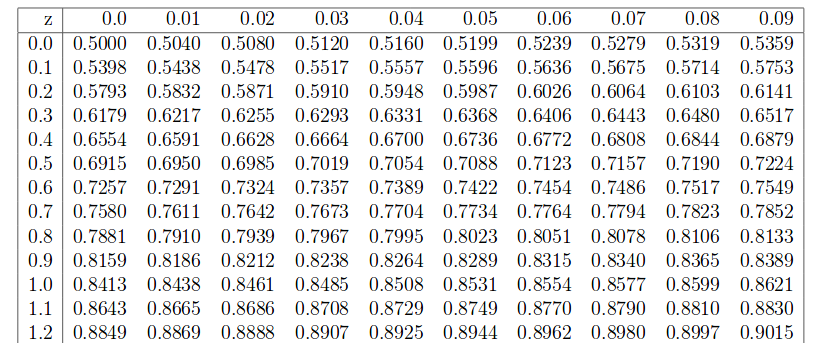
\includegraphics{normal1examen.jpg}

\hypertarget{soluciuxf3n-11}{%
\subsubsection{Solución:}\label{soluciuxf3n-11}}

\(\begin{aligned} P(20< \overline{X}<25 /\overline{X}>20)&=\frac{P(20< \overline{X}<25\cap \overline{X}>20)}{1-P( \overline{X}\leq 20))}\\ &=\frac{F_Z\left(\frac{25-20}{\frac{50}{\sqrt{100}}}\right)-F_Z\left(\frac{20-20}{\frac{50}{\sqrt{100}}}\right)}{1-F_Z\left(\frac{20-20}{\frac{50}{\sqrt{100}}}\right)}= \frac{F_Z(1)-F_Z(0)}{F_Z(0)}. \end{aligned}\)

\hypertarget{ejercicio-13}{%
\subsection{Ejercicio 13}\label{ejercicio-13}}

Lanzamos un dado de 12 caras numeradas con enteros del 1 al 12 sobre una
mesa plana. Observamos el número superior del dado. Suponiendo
equiprobabilidad de todas las caras calcular la probabilidad de que
salga mayor que 8 si el resultado es par. (\emph{1 punto})

\hypertarget{soluciuxf3n-12}{%
\subsubsection{Solución:}\label{soluciuxf3n-12}}

\[ P(X>8/X\in\{2,4,6,8,10,12\})=\frac{P(X\in\{10,12\})}{P(X\in\{2,4,6,8,10,12\})}=\frac{2/12}{6/12}=\frac{1}{3}.\]

\hypertarget{ejercicio-14}{%
\subsection{Ejercicio 14}\label{ejercicio-14}}

Lanzamos una moneda con probabilidad de cara \(p=\frac{1}{2}\) hasta que
sale cara dos veces o bien la hemos lanzamos 5 veces, lo primero que
ocurra.

Denotemos por \(X\) la variable aleatoria que determina el número de
tiradas de la moneda.

Se pide:

a). Describid adecuadamente el espacio muestral de la variable \(X\).
(\textbf{0.5 puntos})

b). Calcular su función de densidad. (\textbf{1 punto})

c). Calcular \(E(X)\). (\textbf{0.5 puntos})

\hypertarget{soluciuxf3n-13}{%
\subsubsection{Solución:}\label{soluciuxf3n-13}}

De notemos los sucesos elementales por \(C\)= cara \(+\)=cruz así el
espacio muestral es

\[\begin{aligned}\Omega=\{&CC,C+C,+CC,++CC,+C+C,C++C,+++CC,++C+C,+C++C,C+++C,\\ & +++++,C++++,+C+++,++C++,+++C+,++++C\}\end{aligned}.\]

Si \(X=\) es l número de tiradas su dominio queda determinado por
\(D_X=\{2,3,4,5\}.\)

Calculemos los valores de su función de probabilidad

\(P(X=2)=\left(\frac{1}{2}\right)^2, P(X=3)=2\cdot\left(\frac{1}{2}\right)^3,P(X=4)=3\cdot\left(\frac{1}{2}\right)^4,P(X=5)=10\cdot \left(\frac{1}{2}\right)^5.\)

\[f_x(x)=P(X=x)= \left\{\begin{array}{ll} 
(x-1)\cdot \left(\frac{1}{2}\right)^x & \mbox{ si } x=2,3,4\\
\frac{10}{32}& \mbox{ si } x=5\\
0 & \mbox{ en el resto de casos.}
\end{array}
\right.
\]

\(E(X)=2\cdot\frac{1}{4}+3\cdot \frac{1}{4}+ 4\cdot \frac{3}{16}+5\cdot \frac{10}{32}=\frac{57}{16}.\)

\hypertarget{ejercicio-15}{%
\subsection{Ejercicio 15}\label{ejercicio-15}}

Sea \(X\) una variable con distribución uniforme en el intervalo
\((1,10)\) con \(a>1\). Consideremos la variable \(Y=\log_{10}(X)\). Se
pide

a). Calcular la función de distribución de \(Y\) (\textbf{1 punto}) b).
Calcular la función de densidad de \(Y\). (\textbf{0.5 puntos}) c).
Calcular el cuantil 0.95 de \(Y\)es decir un valor \(y_0\) tal que
\(P(Y\leq y_0)=0.95\). (\textbf{0.5 puntos})

\hypertarget{soluciuxf3n-14}{%
\subsubsection{Solución:}\label{soluciuxf3n-14}}

Recordemos que \[
F_X(x)=\left\{
\begin{array}{ll} 
0 & \mbox{si} x\leq 0\\
\frac{x-1}{9} & \mbox{si} 0< x < 10\\
1 & \mbox{si} x\geq 10
\end{array}\right.
\]

La variable \(Y\) tendrá por dominio \(D_Y=(0,1)\).

Sea \(y\in(0,1)\) entonces
\(F_Y(y)=P(Y\leq y)=P(\log(X)\leq y)=P(X\leq 10^y)=\frac{10^y-1}{9}\) ya
que como \(0<y<1\) entonces \(0< 10^y < 10\). Así que la función de
distribución es

\[
F_Y(y)=\left\{\begin{array}{ll} 
0 & \mbox{si} x\leq 0\\
\frac{10^y-1}{9} & \mbox{si} 0< y < 1\\
1 & \mbox{si} y\geq 1\\
\end{array}\right.
\]

su densidad es

\[
f_y(y)=F'_Y(y)=\left\{\begin{array}{ll} 
\frac{10^y\cdot log_e(10)}{9} & \mbox{si} 0< y < 1\\
0 & \mbox{en cualquier otro caso}\\
\end{array}\right.
\]

El cuantil \(0.95\) es el valor \(y_0\) tal que
\(F_y(y_0)=P(Y\leq y_0)=0.95\). Por lo tanto

\[F_y(y_0)=\frac{10^{y_0}-1}{9}=0.95\]

así que \(10^{y_0}=9\cdot 0.95+1=9.55\), de donde
\(y_0=\log_{10}(9.55)=0.98.\)

\hypertarget{ejercicio-16}{%
\subsection{Ejercicio 16}\label{ejercicio-16}}

Sea \(X\) una v.a. discreta de dominio \(D_X=\{-2,-1,0,1,2\}\). Sabemos
que \(P(X=x)=p\) para \(x\in D_X\). Calculad \(Var(X)\). (\textbf{0.5
puntos})

\hypertarget{soluciuxf3n-15}{%
\subsubsection{Solución:}\label{soluciuxf3n-15}}

Obviamente \(p=\frac{1}{5}.\)

\(Var(X)=E(X^2)-E(X)^2=\displaystyle\sum_{x=-2}^{2} x^2\cdot P(X=x)-\left(\displaystyle\sum_{x=-2}^2 x\cdot P(X=x)\right)^2= (-2)^2\cdot p+(-1)^2\cdot p+0^2\cdot p+1^2\cdot p+(-2)^2\cdot p-\left(-2\cdot p -1\cdot p+0\cdot p+1\cdot p +2\cdot p\right)^2= 10\cdot p+0^2=10\cdot p=10\cdot \frac{1}{5}=2.\)

\hypertarget{ejercicio-17}{%
\subsection{Ejercicio 17}\label{ejercicio-17}}

Sea \(Z\) una variable aleatoria normal estándar. Tenemos que
`pnorm(-0.2)=0.4207. Calculad \(P(|Z|\geq 0.2)\). (\textbf{0.5 puntos})

\hypertarget{soluciuxf3n-16}{%
\subsubsection{Solución:}\label{soluciuxf3n-16}}

Por simetŕia de la normal estándar sabemos que \(P(Z>0.2)=p(Z<-0.2)\)
por lo tanto

\[P(|Z|\geq 0.2)=P(Z>0.2)+p(Z<-0.2)=2\cdot P(Z<-0.2)=2\cdot 0.4207=
0.8415.\]

Con R

\begin{Shaded}
\begin{Highlighting}[]
\DecValTok{2}\OperatorTok{*}\KeywordTok{pnorm}\NormalTok{(}\OperatorTok{-}\FloatTok{0.2}\NormalTok{)}
\end{Highlighting}
\end{Shaded}

\begin{verbatim}
## [1] 0.8415
\end{verbatim}

\hypertarget{ejercicio-18}{%
\subsection{Ejercicio 18}\label{ejercicio-18}}

\textbf{(3 puntos)} Consideremos la v.a. \(X\) con función densidad

\[f(x)=\left\{
\begin{array}{cl}
 \displaystyle 0.5& \mbox{si } 0< x <1 \\
\displaystyle\frac{x-1}{2} & \mbox{si } 1\leq x < a \\
 \displaystyle 0 & \mbox{ en cualquier otro caso } \\
\end{array}\right..
\]

a). Calculad el valor de \(a\) para que \(f\) sea función de densidad.

b). Para el anterior valor de \(a\) calculad la función de distribución
de \(X\).

c). Para el anterior valor de \(a\) calculad \(E(X)\).

d). Para el anterior valor de \(a\) calculad \(Var(X)\).

\hypertarget{soluciuxf3n-17}{%
\subsubsection{Solución}\label{soluciuxf3n-17}}

Concurso redactar y subir al foro ¡¡¡décimas extra.!!!

\end{document}
